\documentclass{article}

\usepackage{minitoc}
\usepackage{tabularx}
\usepackage{booktabs}
\usepackage{graphicx}
\usepackage{hyperref}
\usepackage{xcolor}
\usepackage{blkarray}
\usepackage{amsthm, amssymb, amsmath}
\usepackage{caption}
\usepackage{subcaption}
\usepackage{multirow}
\usepackage[ruled,vlined]{algorithm2e}

\usepackage{natbib}
\bibliographystyle{abbrvnat}

\theoremstyle{definition}
\newtheorem{definition}{Definition}[section]
\newtheorem{theorem}{Theorem}[section]
\newtheorem{lemma}[theorem]{Lemma}

\usepackage[margin=2.5cm, includefoot, footskip=30pt]{geometry}
\pagestyle{plain}
\setlength{\parindent}{0em}
\setlength{\parskip}{1em}

\renewcommand{\baselinestretch}{1}

\newcommand{\nikoleta}[1]{\textcolor{orange}{{\bf NG:} #1}}

\newtheorem{proposition}{Proposition}

\title{$n-$bits reactive strategies in repeated games}

\author{Nikoleta E. Glynatsi, Christian Hilbe, Martin Nowak}
\date{}

\begin{document}

\maketitle

\section{Introduction}

In this work we explore \textit{reactive strategies} in the infinitely repeated
prisoner's dilemma. The prisoner's dilemma is a two person symmetric game that
provides a simple model of cooperation. Each of the two players, \(p\) and
\(q\), simultaneously and independently decide to cooperate (\(C\)) or to defect
(\(D\)). A player who cooperates pays a cost \(c > 0\) to provide a benefit
\(b > c\) for the co-player. A cooperator either gets \(b - c\) (if the
co-player also cooperates) or \(-c\) (if the co-player defects). A defector either gets
\(b\) or 0, and thus, the payoffs of player \(p\) take the form,

\begin{equation}\label{eq:donation_payoffs}
  \begin{blockarray}{ccc}
      & \text{cooperate} & \text{defect} \\
      \begin{block}{c(cc)}
          \text{cooperate} & b - c & -c \\
          \text{defect} & c & 0 \\
      \end{block}
  \end{blockarray}
\end{equation}

The transpose of the matrix (\ref{eq:donation_payoffs}) are the payoffs of
co-player \(q\). Alternatively, we can define each player's payoffs as vectors
by,

\begin{equation}\label{eq:vector_payoffs}
  \mathbf{S}_{p} = (b-c, -c, b, 0) \quad \textrm{and} \quad  \mathbf{S}_{q} = (b - c, b, -c, 0).
\end{equation}

We study the infinitely repeated prisoner's dilemma. The infinitely repeated
prisoner's dilemma consists of an infinite number of repetitions of the
prisoner's dilemma (called the stage game).

\subsection{Strategies}

A strategy is a mapping from the entire history of play to an action of the
stage game, and for the repeated prisoner's dilemma there are infinitely many
strategies. Here we focus on \textit{\(n-\)bit reactive strategies}; a special case of
\textit{memory-\(n\) strategies}. \(n-\)bit reactive strategies
only respond to the co-player's previous \(n\) moves,
whereas memory-\(n\) strategies take into account their own and the co-player's
previous \(n\) moves.

Memory-\(n\) strategies are very well studied in the
literature~\citep{baek:scientific:2016, hilbe:PNAS:2017,
glynatsi:scientific:2020, press:PNAS:2012, stewart:scientific:2016} with a major
focus on memory-one strategies. Memory-one strategies consider only the outcome
of the previous stage game to decide on an action, and have gained their
attention mainly due to the mathematical tractability.

There are four possible outcomes to a one stage prisoner's dilemma, and with the
outcomes listed in order as \(CC, CD, DC, DD\), a memory-one strategy for \(p\)
is a vector \(\mathbf{p} = (p_1, p_2, p_3, p_4)\) where \(p_i\) is the
probability of playing \(C\) when the \(i^{\text{th}}\) outcome occurred in the
previous round. A play between two memory-one strategies, \(\mathbf{p} = (p_1,
p_2, p_3, p_4)\) and \(\mathbf{q} = (q_1, q_2, q_3, q_4)\), follows a Markov
chain with four states, corresponding to the four possible outcomes, and with
the transition matrix \(M\). The invariant distribution \(\mathbf{v}\) is the
solution to \(\mathbf{v} M = \mathbf{v}\), and it gives the probabilities that
the players are in any of the states in the long run of the game.

\begin{equation}
\displaystyle M_1 = \left[\begin{matrix}p_{1} q_{1} & p_{1} \left(1 - q_{1}\right) & q_{1} \left(1 - p_{1}\right) & \left(1 - p_{1}\right) \left(1 - q_{1}\right)\\
  p_{2} q_{3} & p_{2} \left(1 - q_{3}\right) & q_{3} \left(1 - p_{2}\right) & \left(1 - p_{2}\right) \left(1 - q_{3}\right)\\
  p_{3} q_{2} & p_{3} \left(1 - q_{2}\right) & q_{2} \left(1 - p_{3}\right) & \left(1 - p_{3}\right) \left(1 - q_{2}\right)\\
  p_{4} q_{4} & p_{4} \left(1 - q_{4}\right) & q_{4} \left(1 - p_{4}\right) & \left(1 - p_{4}\right) \left(1 - q_{4}\right)\end{matrix}\right].
\end{equation}

It is a known result that given the invariant distribution we can calculate the expected payoffs for
each player, \(s_{\mathbf{p}}\) and \(s_{\mathbf{q}}\), as follows

\begin{equation*}
  \pi(\mathbf{p}, \mathbf{q}) = \mathbf{v} \cdot \mathbf{S}_{p} \text{ and } \pi(\mathbf{q}, \mathbf{p}) = \mathbf{v} \cdot \mathbf{S}_{q}.
\end{equation*}

As previously mentioned, reactive strategies are a subset of memory-\(n\)
strategies, and consequently, one-bit reactive strategies are a subset of
memory-one strategies. One-bit reactive strategies consider only the co-player's
last action. Thus, a one-bit strategy treats the outcomes \(CC\) and \(CD\) as
the same; the co-player cooperated in the last turn. In this case \(p_1 = p_3\).
Similarly, the probabilities of cooperating given that the co-player defected in
the last turn are the same regardless of the strategy's own action; \(p_2 = p_4\),
and so \(\mathbf{p} = (p_1, p_2, p_1, p_2)\). The methodology we have outlined
here also applies to one-bit reactive strategies.

Reactive strategies have some attention in the
literature~\citep{sigmund:JTB:1989, wahl:JTB:1999}, however, the majority of
work focuses on one-bit reactive strategies. Even though for memory-\(n\)
strategies previous work have shown that we can characterize Nash equilibria for
an arbitrary memory size~\citep{hilbe:PNAS:2017, stewart:scientific:2016} no
similar work has been done on reactive strategies. The work
of~\citep{hilbe:PNAS:2017} have shown that in the case of memory-\(n\)
strategies, more memory allows for more cooperation to evolve. We test this
hypothesis in the case of reactive strategies. Previous
work~\citep{baek:scientific:2016} have compared memory-\(n\) to reactive
strategies, however, this was done for low memory strategies. The aim of this
work is to extensively study reactive strategies of higher memory. We want to
contribute to the ongoing discussions on (1) the effects of more memory on
cooperation (2) the difference between memory-\(n\) strategies and reactive
ones.

In section~\ref{section:good_nash_strategies} we analytically characterize
reactive strategies that are of Nash type and cooperative. In
section~\ref{section:pure_strategies} we show that pure \(n-\)bit reactive
strategies can not can not sustain a cooperative Nash equilibrium. Finally, in
section~\ref{section:evolutionary_simulations} we perform an evolutionary analysis, and investigate which strategies
evolve.

\section{Results}

\subsection{Cooperative Nash for Two-bit reactive strategies}\label{section:good_nash_strategies}

\subsubsection{Good \(n\)-bit reactive strategies}

In~\citep{akin:EGADS:2016}, Akin gives the following definitions for memory-one
strategies.

\begin{definition}
A memory-one strategy is \textbf{agreeable} if it always cooperates following a mutual cooperation,
thus \(p_1=1\).
\end{definition}

\begin{definition}
  A strategy for \(p\) is called \textbf{good} if (i) it is agreeable,
  and (ii) if for any general strategy chosen by \(q\) against it the expected
  payoffs satisfy:
  
  \begin{equation}
    s_{\mathbf{q}} \geq (b - c) \Rightarrow s_{\mathbf{q}} = s_{\mathbf{p}} =  (b - c).
  \end{equation}

  The strategy is of \textbf{Nash type} if (i) it is agreeable and (ii) if the
  expected payoffs against any \(q\) general strategy satisfy:

  \begin{equation}
    s_{\mathbf{q}} \geq R \Rightarrow s_{\mathbf{q}} =  (b - c).
  \end{equation}
\end{definition}

Hence, a strategy is good if the co-player achieves the reward payoff if and
only if the focal player does as well. A Nash type strategy reassures that the
co-player can never receive a payoff higher than \(b - c\).

Notice that the definitions of good and Nash make no assumptions regarding the type of
strategies the players need to play, and thus, these are extendable to \(n-\)
bit reactive strategies. The notion of agreeable strategies is generalized
in the case of reactive strategies as follows.

\begin{definition}\label{def:agreeable}
A \(n-\)bit reactive strategy is agreeable if it cooperates with a probability one
given that the co-player has consecutively cooperated in that last \(n\) rounds.
\end{definition}

Following the introduction of these concepts, Akin proves
Theorem~\ref{theorem:akin} which he uses to characterize all memory-one
strategies that are of \textit{Nash type} and \textit{good}.

\begin{theorem}{Akin's Theorem.}
  Assume that player \(p\) uses the memory-one strategy \(\mathbf{\tilde{p}} = \mathbf{p} - \mathbf{e}_{12}\) where
  \(\mathbf{e}_{12} = (1, 1, 0, 0)\), and \(q\) uses a strategy that leads to a sequence
  of distributions \(\{\mathbf{v}^{(n)}, n = 1, 2, ...\}\) with \(\mathbf{v}^{(k)}\) representing the
  distribution over the states in the \(k^{\text{th}}\) round of the game. Let
  \(\mathbf{v}\) be an associated stationary distribution. Then,

  \begin{align}
    \lim_{n \rightarrow \infty} \frac{1}{n} \sum_{k=1}^{n} \mathbf{v}^{(n)} \cdot \mathbf{\tilde{p}} = 0, \text{ and therefore } \mathbf{v} \cdot \mathbf{\tilde{p}} = 0.
  \end{align}
\end{theorem}\label{theorem:akin}

Akin's theorem is extendable to higher memory strategies; we demonstrate this for
the special case of two-bit reactive strategies.

\subsubsection{Two-bit reactive strategies}

In the case of \textit{two-bit reactive strategies}, players consider the last
two actions of the co-player.  Since for a single round there are 4 possible
outcomes, for two rounds there will be 16 \((4 \times 4)\). We denote the
possible outcomes as \(E_p E_q | F_p F_q\) (\(E_p, E_q, F_p, F_q \in \{C, D\}\))
where the outcome of the previous round is \(E_p E_q\) and the outcome of the
current round is \(F_p F_q\). With the outcomes listed in order as \(CC|CC,
CC|CD, \dots, DD|DC, DD|DD\) a two-bit reactive strategy for \(p\) is a vector
\(\mathbf{p} = (p_1, p_2, p_1, p_2, p_3, p_4, p_3, p_4, p_1, p_2, p_1, p_2, p_3,
p_4, \allowbreak p_3, p_4)\) where

\begin{itemize}
  \item \(p_1\) is the probability of playing \(C\) when the last two actions of the co-player were \(CC\),
  \item \(p_2\) is the probability of playing \(C\) when the last two actions of the co-player were \(CD\),
  \item \(p_3\) is the probability of playing \(C\) when the last two actions of the co-player were \(DC\),
  \item \(p_4\) is the probability of playing \(C\) when the last two actions of the co-player were \(DD\).
\end{itemize}

For simplicity, we denote a two-bit reactive strategy for \(p\) as
\(\mathbf{\hat{p}} = (p_1, p_2, p_3, p_4)\).

The play between two two-bits reactive strategies can be described by a Markov
process with the transition matrix \(\tilde{M}\).

\resizebox{\linewidth}{!}{%
$
\tilde{M} = \left(\begin{array}{cccccccccccccccc}
 p_1 q_1 & p_1 (1-q_1) & (1-p_1) q_1 & (1-p_1) (1-q_1) & 0 & 0 & 0 & 0 & 0 & 0 & 0 & 0 & 0 & 0 & 0 & 0 \\
 0 & 0 & 0 & 0 & p_2 q_1 & p_2 (1-q_1) & (1-p_2) q_1 & (1-p_2) (1-q_1) & 0 & 0 & 0 & 0 & 0 & 0 & 0 & 0 \\
 0 & 0 & 0 & 0 & 0 & 0 & 0 & 0 & p_1 q_2 & p_1 (1-q_2) & (1-p_1) q_2 & (1-p_1) (1-q_2) & 0 & 0 & 0 & 0 \\
 0 & 0 & 0 & 0 & 0 & 0 & 0 & 0 & 0 & 0 & 0 & 0 & p_2 q_2 & p_2 (1-q_2) & (1-p_2) q_2 & (1-p_2) (1-q_2) \\
 p_3 q_1 & p_3 (1-q_1) & (1-p_3) q_1 & (1-p_3) (1-q_1) & 0 & 0 & 0 & 0 & 0 & 0 & 0 & 0 & 0 & 0 & 0 & 0 \\
 0 & 0 & 0 & 0 & p_4 q_1 & p_4 (1-q_1) & (1-p_4) q_1 & (1-p_4) (1-q_1) & 0 & 0 & 0 & 0 & 0 & 0 & 0 & 0 \\
 0 & 0 & 0 & 0 & 0 & 0 & 0 & 0 & p_3 q_2 & p_3 (1-q_2) & (1-p_3) q_2 & (1-p_3) (1-q_2) & 0 & 0 & 0 & 0 \\
 0 & 0 & 0 & 0 & 0 & 0 & 0 & 0 & 0 & 0 & 0 & 0 & p_4 q_2 & p_4 (1-q_2) & (1-p_4) q_2 & (1-p_4) (1-q_2) \\
 p_1 q_3 & p_1 (1-q_3) & (1-p_1) q_3 & (1-p_1) (1-q_3) & 0 & 0 & 0 & 0 & 0 & 0 & 0 & 0 & 0 & 0 & 0 & 0 \\
 0 & 0 & 0 & 0 & p_2 q_3 & p_2 (1-q_3) & (1-p_2) q_3 & (1-p_2) (1-q_3) & 0 & 0 & 0 & 0 & 0 & 0 & 0 & 0 \\
 0 & 0 & 0 & 0 & 0 & 0 & 0 & 0 & p_1 q_4 & p_1 (1-q_4) & (1-p_1) q_4 & (1-p_1) (1-q_4) & 0 & 0 & 0 & 0 \\
 0 & 0 & 0 & 0 & 0 & 0 & 0 & 0 & 0 & 0 & 0 & 0 & p_2 q_4 & p_2 (1-q_4) & (1-p_2) q_4 & (1-p_2) (1-q_4) \\
 p_3 q_3 & p_3 (1-q_3) & (1-p_3) q_3 & (1-p_3) (1-q_3) & 0 & 0 & 0 & 0 & 0 & 0 & 0 & 0 & 0 & 0 & 0 & 0 \\
 0 & 0 & 0 & 0 & p_4 q_3 & p_4 (1-q_3) & (1-p_4) q_3 & (1-p_4) (1-q_3) & 0 & 0 & 0 & 0 & 0 & 0 & 0 & 0 \\
 0 & 0 & 0 & 0 & 0 & 0 & 0 & 0 & p_3 q_4 & p_3 (1-q_4) & (1-p_3) q_4 & (1-p_3) (1-q_4) & 0 & 0 & 0 & 0 \\
 0 & 0 & 0 & 0 & 0 & 0 & 0 & 0 & 0 & 0 & 0 & 0 & p_4 q_4 & p_4 (1-q_4) & (1-p_4) q_4 & (1-p_4) (1-q_4) \\
\end{array}\right).$}

Note that from state \(CC|CC\) only the states \(CC|CC, CC|CD, CC|DC, CC|DD\)
are reachable. That is because the current outcome \(F_p F_q\) in this state has
to match the previous outcome \(E_p E_q\) in the ``next'' state. Thus, in each
row of the matrix there will be at most four non-zero elements. The invariant
distribution \(\mathbf{\tilde{v}}\) is the solution to \(\mathbf{\tilde{v}}
\tilde{M} = \mathbf{\tilde{v}}\).

In the infinitely repeated prisoner's dilemma, the probability that two players
are in a \(CC\) state in the last round is the same as the probability of them
being in a \(CC\) in the second to last round, thus, the following holds for
\(\mathbf{\tilde{v}}\),

\begin{align}
  \sum_{i, j \in \{C, D\}} \tilde{v}_{i, j | CD} & = \sum_{i, j \in \{C, D\}} \tilde{v}_{CD | ij}.
\end{align}

The extension to Akin's Theorem (Theorem~\ref{theorem:akin}) is give by
Lemma~\ref{lemma:akin_extended}.

\begin{lemma}\label{lemma:akin_extended}
  Assume that player \(p\) uses a two-bit reactive strategy \(\mathbf{\tilde{p}} = \mathbf{p} - \mathbf{e}_{i \in \{1, 2,
  5, 6, 9, 10, 13, 14\}}\), and \(q\) uses a strategy that leads to a sequence
  of distributions \(\{\mathbf{\tilde{v}}^{(n)}, n = 1, 2, ...\}\) with
  \(\mathbf{\tilde{v}}^{(k)}\) representing the distribution over the states in the
  \(k^{\text{th}}\) round of the game. Let \(\mathbf{\tilde{v}}\) be an associated
  stationary distribution. Then

  \begin{align*}
    \lim_{n \rightarrow \infty} \frac{1}{n} \sum_{k=1}^{n} \mathbf{\tilde{v}}^{(n)} \cdot\mathbf{\tilde{p}} & = 0, \text{ and therefore } \mathbf{\tilde{v}} \cdot \mathbf{\tilde{p}} = 0.
  \end{align*}

  \begin{align}\label{eq:akin_extended}
  \mathbf{\tilde{v}}^{(n)} \cdot \mathbf{\tilde{p}} = 0 \Rightarrow & \nonumber \\
  & (\tilde{v}_{1} + \tilde{v}_{9}) (1 - p_1) + (\tilde{v}_{2} + \tilde{v}_{10}) (1 - p_2)  + (\tilde{v}_{5} + \tilde{v}_{13}) (1 - p_3) + (\tilde{v}_{6} + \tilde{v}_{14}) (1 - p_4) \nonumber \\
  & + (\tilde{v}_{3} + \tilde{v}_{11})p_1  + (\tilde{v}_{4} + \tilde{v}_{12})p_2 + (\tilde{v}_{7} + \tilde{v}_{15}) p_3 + (\tilde{v}_{8} + \tilde{v}_{16}) p_4 = 0.
  \end{align}
\end{lemma}

\begin{proof}
  The probability that \(p\) cooperates in the \(n^{\text{th}}\) round, denoted
  by \(\tilde{v}_{\text{C}}^{(n)}\), is \(\tilde{v}_{\text{C}}^{(n)} = \tilde{v}_{1}^{(n)} +
  \tilde{v}_{2}^{(n)} + \tilde{v}_{5}^{(n)} + \tilde{v}_{6}^{(n)} + \tilde{v}_{9}^{(n)} +  \tilde{v}_{10}^{(n)} +
  \tilde{v}_{13}^{(n)} + \tilde{v}_{14}^{(n)} = \mathbf{\tilde{v}} \cdot \mathbf{e}_{i \in \{1, 2,
  5, 6, 9, 10, 13, 14,\}}\). The probability that \(p\) cooperates in the
  \((n + 1)^{th}\) round, denoted by \(\tilde{v}_{\text{C}}^{(n + 1)}\) = \(\tilde{v}^{(n)} \cdot \mathbf{p}\).
  Thus,

  \begin{equation*}
   \tilde{v}_{\text{C}}^{(n + 1)} - \tilde{v}_{\text{C}}^{(n)} = \mathbf{\tilde{v}^{(n)}} \cdot \mathbf{p} - \mathbf{\tilde{v}} \cdot \mathbf{e}_{i \in \{1, 2,
    5, 6, 9, 10, 13, 14\}} = \mathbf{\tilde{v}^{(n)}} \cdot (\mathbf{p} - \mathbf{e}_{i \in \{1, 2,
    5, 6, 9, 10, 13, 14\}}) = \mathbf{\tilde{v}}^{(n)} \cdot \mathbf{\tilde{p}}.
  \end{equation*}

  This implies \(\tilde{v}_{\text{C}}^{(n + 1)} - \tilde{v}_{\text{C}}^{(n)}
  = \sum_{k=1}^{n} (\tilde{v}_{\text{C}}^{(k + 1)} - \tilde{v}_{\text{C}}^{(k)})
  = \sum_{k=1}^{n} (\mathbf{\tilde{v}}^{(k)} \cdot \mathbf{\tilde{p}})\). Since
  \(0 \leq \tilde{v}_{\text{C}}^{(k)} \geq 1\) for any \(k\),

  \begin{equation*}
    \lim_{n \rightarrow \infty} \frac{1}{n} \sum_{k=1}^{n} \mathbf{\tilde{v}}^{(k)} \cdot \mathbf{\tilde{p}} = 
    \lim_{n \rightarrow \infty} \frac{1}{n} \sum_{k=1}^{n} (\tilde{v}_{\text{C}}^{(n + 1)} - \tilde{v}_{\text{C}}^{(1)}) = 0.
  \end{equation*}

  For the stationary distribution \(\mathbf{\tilde{v}}\) that is the limit of
  some subsequence of the Cesaro averages \(\{\frac{1}{n} \sum_{k=1}^{n} \mathbf{\tilde{v}}^{(k)}\}\),
  the continuity of the dot product implies \(\mathbf{\tilde{v}} \cdot \mathbf{\tilde{p}} = 0 \)

\end{proof}

We know that the invariant distribution combined with the payoff vectors give
the expected payoffs for each player. In the case of the two-bit reactive
strategies there can be two set of payoff vectors; (1) the payoffs are
defined based on the outcome of the last round,

\begin{equation}\label{eq:last_round_two_bits}
  \begin{array}{*{16}{c}}
    \mathbf{S}_{p} = ( b - c , & -c , & b , & 0 , & b - c , & -c , & b , & 0 , & b - c , & -c , & b , & 0 , & b - c , & -c , & b , & 0)  \;, \\
    \mathbf{S}_{q} = ( b - c, & b, & -c, & 0, & b - c, & b, & -c, & 0, & b - c, & b, & -c, & 0, & b - c, & b, & -c, & 0).
  \end{array}
\end{equation}

(2) the payoffs are defined based on the outcome of the second to last round,

\begin{equation}\label{eq:second_to_last_round_two_bits}
  \begin{array}{*{16}{c}}
    \mathbf{S}'_{p} = (b - c, & b - c, & b - c, & b - c, & -c, & -c, & -c, & -c, & b, & b, & b, & b, & 0, & 0, & 0, & 0)  \;, \\
    \mathbf{S}'_{q} = (b - c, & b - c, & b - c, & b - c, & b, & b, & b, & b, & -c, & -c, & -c, & -c, & 0, & 0, & 0, & 0).
  \end{array}
\end{equation}

Note that \(\mathbf{s_{p}} = \mathbf{\tilde{v}} \times \mathbf{S}_{p} =
\mathbf{\tilde{v}} \times \mathbf{S}'_{p}\) and \(\mathbf{s_{q}} =\mathbf{\tilde{v}}
\times \mathbf{S}_{q} = \mathbf{\tilde{v}} \times \mathbf{S}'_{q}\). From
hereupon we consider the payoff vectors \(\mathbf{S}_{p}\) and
\(\mathbf{S}_{q}\) unless stated otherwise.

\subsubsection{Good and Nash type two-bit reactive strategies}

We are interested in which two-bit reactive strategies can sustain a Nash
equilibrium, and more specifically, a good/cooperative one. An agreeable strategy in
the case of two-bit reactive strategies is a play that always cooperates after
two consecutive cooperations of the co-player, thus \(p_1 = 1\).

\begin{theorem}

Let the two-bit reactive strategy \(\mathbf{\hat{p}} = (p_{1}, p_{2}, p_{3}, p_{4})\) be an \textbf{agreeable
strategy}; that is \(p_1 = 1\). Strategy \(\mathbf{\hat{p}}\) is \textbf{Nash} if the
following inequalities hold:
\begin{equation*}
    p_4 \leq 1 - \frac{c}{b} \qquad  p_2  \leq p_4 \qquad p_3 \leq 1 \qquad (1 + p_2) \leq \frac{b}{c} - \frac{p_4 (b - c)}{c}
\end{equation*}

The agreeable strategy \(\mathbf{\hat{p}}\) is good if and only if both inequalities above are strict.
\end{theorem}

\begin{proof}
We first eliminate the possibility \(p_4 = 1\). If \(p_4 = 1\), then \(\mathbf{\hat{p}}
= (1, p_2, p_3, 1)\). If against this \(q\) plays AllD \(= (0, 0, 0, 0)\),
then \(\{CD\}\) is a terminal set and so
with \(s_\mathbf{q} = b\) and \(s_\mathbf{p} = -c\). Hence, \(\mathbf{\hat{p}}\) is not of Nash type.

We now assume \(1 - p_4 > 0\). Observe that

\begin{align}\label{eq:nash_condition_last_round}
  s_\mathbf{q} - (b - c) & = \mathbf{\tilde{v}} \times \mathbf{S}_{q} - (b - c) \sum_{i=1}^{16} \tilde{v}_{i}\\ \nonumber
  & = (\tilde{v}_{2} + \tilde{v}_{6} + \tilde{v}_{10} + \tilde{v}_{14}) c + (c - b) (\tilde{v}_{4} + \tilde{v}_{8} + \tilde{v}_{12} + \tilde{v}_{16}) - b (\tilde{v}_{3} + \tilde{v}_{7} + \tilde{v}_{11} + \tilde{v}_{15}) .
\end{align}

Multiplying by the positive quantity \((1 - p_4)\) and collecting terms, we have

\begin{align}
  s_\mathbf{q} \geq (b - c) & \Rightarrow \\ \nonumber
  (1 - p_4)(\tilde{v}_{6} + \tilde{v}_{14}) c & \geq  - c(1 - p_4)(\tilde{v}_{2} + \tilde{v}_{10}) + (1 - p_4)(-c + b) (\tilde{v}_{4} + \tilde{v}_{8} + \tilde{v}_{12} + \tilde{v}_{16}) + b (1 - p_4) (\tilde{v}_{3} + \tilde{v}_{7} + \tilde{v}_{11} + \tilde{v}_{15}) .
\end{align}

Since \(\tilde{p_1} = 0\), equation (\ref{eq:akin_extended}) implies

\[(1 - p_2)
(\tilde{v}_{10} + \tilde{v}_{2}) + (1 - p_3) (\tilde{v}_{13} + \tilde{v}_{5}) +  (1 - p_4) (\tilde{v}_{14} + \tilde{v}_6)
- p_2 (\tilde{v}_{12} + \tilde{v}_4) - p_3 (\tilde{v}_{15} + \tilde{v}_7) - p_4 (\tilde{v}_{16} + \tilde{v}_{8}) - \tilde{v}_{11} - \tilde{v}_{3} = 0,\]
and so,
\[(1 - p_4) (\tilde{v}_{14} + \tilde{v}_6) = - ((1 - p_2)
(\tilde{v}_{10} + \tilde{v}_{2}) + (1 - p_3) (\tilde{v}_{13} + \tilde{v}_{5}) 
- p_2 (\tilde{v}_{12} + \tilde{v}_4) - p_3 (\tilde{v}_{15} + \tilde{v}_7) - p_4 (\tilde{v}_{16} + \tilde{v}_{8}) - \tilde{v}_{11} - \tilde{v}_{3}).\]

Substituting in the above inequality and collecting terms we get

\begin{align}
  & A (\tilde{v}_{10} + \tilde{v}_{2}) + B (\tilde{v}_{12} + \tilde{v}_4) 
  + C (\tilde{v}_{13} + \tilde{v}_5) + D (\tilde{v}_{15} + \tilde{v}_7) + E (\tilde{v}_{11} + \tilde{v}_{16} + \tilde{v}_3 + \tilde{v}_8) \geq  0 \label{eq:nash_condition_special_case} \\ \text{ with } \nonumber \\ 
  & \qquad A = (c (p_2 - p_4)), \qquad B = (c (1 + p_2 - p_4) + b (-1 + p_4)), \qquad C = ( c (-1 + p_3)),  \nonumber \\
  & \qquad  \qquad  \qquad \qquad \qquad D = (c p_3 + b (-1 + p_4)), \qquad E = c + 
  b (-1 + p_4). \nonumber
\end{align}

In the case where \(A, B, C, D\) and \(E\) are smaller than 0, condition
(\ref{eq:nash_condition_special_case}) holds iff \(\tilde{v}_2, \tilde{v}_3,
\tilde{v}_4, \tilde{v}_5, \tilde{v}_7, \tilde{v}_8, \tilde{v}_{10},
\tilde{v}_{11}, \tilde{v}_{12}, \tilde{v}_{13}, \tilde{v}_{15}, \tilde{v}_{16} =
0\). This implies, that \((\tilde{v}_1 + \tilde{v}_9) (1 - p_1) + (\tilde{v}_6 +
\tilde{v}_{14}) (1 - p_4) = 0\). \(p_4\) can not be 1, thus \(\tilde{v}_6,
\tilde{v}_{14} = 0\). This means \((\tilde{v}_1 + \tilde{v}_9) = 1\), so both
players receive the reward payoff and \(\mathbf{\hat{p}}\) is good.

For \(A, B, C, D, E \leq 0\) we derive the following conditions,

\begin{align}\label{eq:nash_conditions}
  p_4       & \leq 1 - \frac{c}{b} \\
  p_2       & \leq p_4 \\
  p_3       & \leq 1 \\
  (1 + p_2) & \leq \frac{b}{c} - \frac{p_4 (b - c)}{c}
\end{align}

\end{proof}

\nikoleta{The code for getting these conditions is in `src/mathemtica/Two bit reactive.nb`.}

We can also explore the space of two-bit reactive strategies numerically. For a
random agreeable two-bit reactive strategy we can evaluate if it's Nash using
the Algorithm~\ref{algorithm:numerical_nash}.

\begin{algorithm}[H]
  \SetAlgoLined \For{ $i <$ maximum number of points}{\(\mathbf{\hat{p}}\)
   $\leftarrow$ random: $\{\emptyset \}\ \rightarrow R_{[0, 1]}^4$\;
   \(p_1\)
   $\leftarrow$ 1\;
   $L(\mathbf{\hat{p}}) = \{\mathbf{\hat{q}} \,|\, \pi(\mathbf{\hat{p}}, \mathbf{\hat{p}}) \geq \pi(\mathbf{\hat{q}}, \mathbf{\hat{p}}) \text{ for } \mathbf{\hat{q}} \in \{\mathbf{\hat{q}_i} \in P([0, 1]) \,|\, |\mathbf{\hat{q}_i}| = 16 \}\}$\;
  \uIf{$ L(\mathbf{\hat{p}}) = \emptyset $}{
    isNash $\leftarrow$ True \;
  }
  \Else{
    isNash $\leftarrow$ False \;
  }
  \Return (\(\mathbf{\hat{p}}\), isNash) \;}
  \caption{Numerical evaluation for Nash.}\label{algorithm:numerical_nash}
\end{algorithm}

\(\{\mathbf{\hat{q}_i} \in P([0, 1]) \,|\, |\mathbf{\hat{q}_i}| = 16 \}\) is
the set of all pure two-bit reactive strategies.

For a given set of parameter values (\(b=2 \text{ and } c=1\)) we can illustrate
the space of provably Nash, Figure~\ref{fig:two_bit_reactive_nash_results}A. The
results of the numerical evaluation are shown in
Figures~\ref{fig:two_bit_reactive_nash_results}B - C. As a proof of concept, the
numerical evaluation confirms that the points which satisfy conditions
(\ref{eq:nash_conditions}) are indeed Nash. However, we can also observe
that there are points in the two-bit space which are Nash that do not satisfy
the conditions. Thus, conditions (\ref{eq:nash_conditions}) are sufficient for
Nash but they are not absolute. The final conclusion is that for a point to be Nash
we do not need to check against all 16 pure two-bit strategies but only against
two; AllD and N6\(=(0, 1, 1, 0)\). Akin showed a similar result
in~\citep{akin:EGADS:2016}.


\begin{figure}[!htbp]
     \centering
     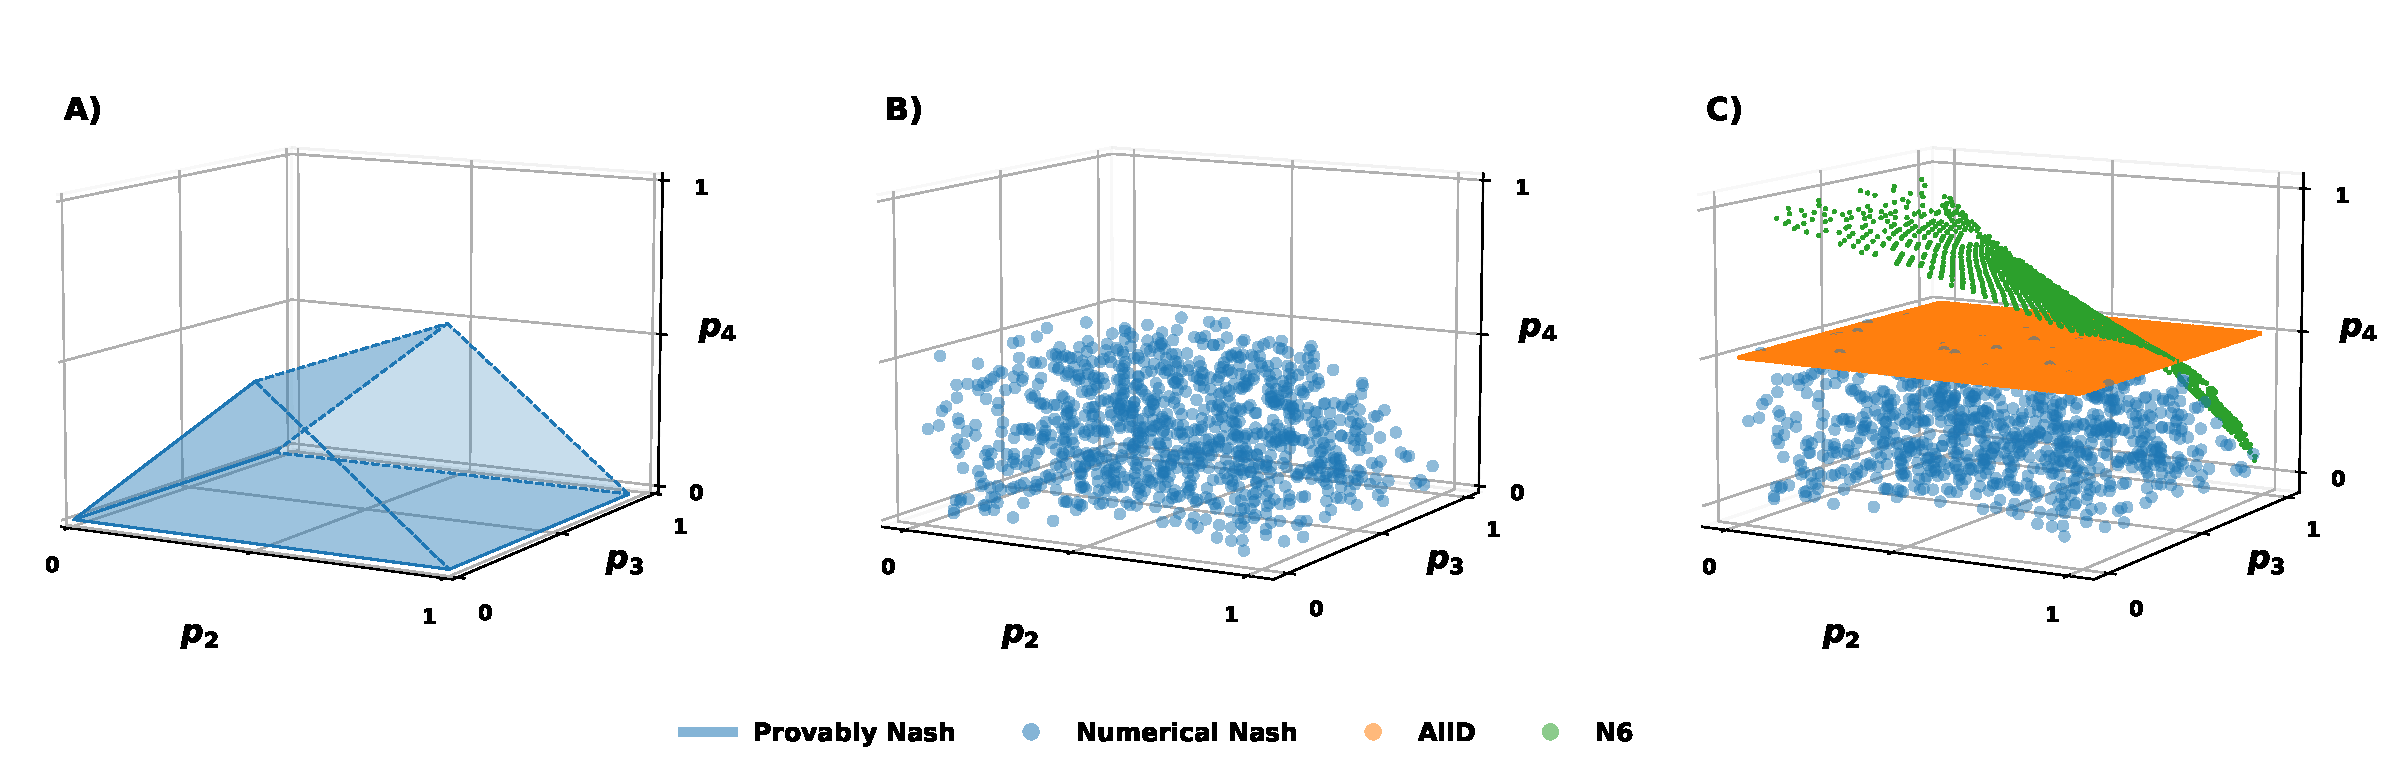
\includegraphics[width=\textwidth]{static/two_bit_results.pdf}
     \caption{\textbf{Nash results for two-bit strategies.}
     \textbf{A) Provably Nash.} We have shown that if a two-bit reactive Nash is
     within this space, thus satisfy conditions (\ref{eq:nash_conditions}), then
     it is Nash. \textbf{B) Numerical Nash.} The results from
     Algorithm~\ref{algorithm:numerical_nash}. We evaluated \(10 ^ 5\) points in
     the space and here we are plotting 1000 randomly selected points. \textbf{C)
     The numerical results including the surfaces for AllD and N6.} The
     numerical results have shown that there are two pure strategies for which
     we have to check against to verify Nash. The planes are the planes for
     \(\pi(\mathbf{\hat{p}}, \mathbf{\hat{p}}) - \pi(\mathbf{\hat{q}_i},
     \mathbf{\hat{p}}) = 0\) where \(\mathbf{\hat{p}}\) is a generic agreeable
     two-bit reactive strategy and \(\mathbf{\hat{q}_i} \in \{\text{AllD, N6}\}\).
     Note that we do
     not plot \(p_1\), as \(p_1=1\). Parameters: \(c=1,
     b=2\).}\label{fig:two_bit_reactive_nash_results}
\end{figure}

\nikoleta{The code for getting the plots is in `nbs/Two bit reactive Nash`.}

\subsubsection{Some further thoughts}

We have also performed the numerical evaluation for the prisoner's dilemma using
the payoff matrix,

\begin{equation}
  \begin{blockarray}{ccc}
      & \text{cooperate} & \text{defect} \\
      \begin{block}{c(cc)}
          \text{cooperate} & R & 0 \\
          \text{defect} & 1 & P \\
      \end{block}
  \end{blockarray}
\end{equation}

with \(R=0.6\) and \(P=0.1\). Though the results mainly remain similar, in the
case of the prisoner's dilemma and for the given values, checking for Nash only
against two strategies is not enough. In this case we also need to check for N7
which is the pure strategy given by \((0, 1, 1, 1)\).

\nikoleta{This is demonstrated in `nbs/Two bit reactive Nash`.}

Another thought. Two-bit reactive strategies are a specific case of memory-two
strategies. The steps that we have taken in this section can also be applied to
the case of memory-two strategies. However, now the strategies are 16
dimensional. Regardless, we can obtain some conditions.

\nikoleta{This is demonstrated in `src/mathematica/Memory\_two.nb`.}

We expect that the methodology can be applied to \(n-\)bit reactive strategies
and memory-\(n\) strategies. However, we expect that the space that we can prove
is Nash is smaller and smaller in the feasible space of these strategies.

\subsection{Pure \(n-\)bit Reactive Strategies with Errors}\label{section:pure_strategies}

In this section we perform a numerical analysis to identify all strict Nash
equilibria if players are restricted to pure strategies. To this end, we use a
method defined by the work~\citep{hilbe:PNAS:2017} which we will refer to as the
Vaquero method. The method numerically identifies all (strict) Nash equilibria
among a finite set of strategies, and moreover it returns for which parameter
values the respective strategy is Nash. In our case we use the donation game
thus the method returns which benefit-to-cost ratio \(\frac{b}{c}\) is required
for a strategy to be Nash.

\subsubsection{The Vaquero Method}

Let \(p\) and \(q\) play as \(\mathbf{p}_{\epsilon}\) and
\(\mathbf{q}_{\epsilon}\) from a given set of strategies in a noisy environment
with \(\epsilon > 0\) where \(\mathbf{p}_{\epsilon} = \epsilon(1 - \mathbf{p}) +
(1 - \epsilon)\mathbf{p} \). Given the two strategies we numerically compute
the three following measures:


\begin{itemize}
  \item The fraction of rounds \(\rho\) in which player \(p\) cooperates against itself.
  \item The fraction of rounds \(\tilde{\rho}_p\) in which player \(p\) cooperates against \(q\).
  \item The fraction of rounds \(\tilde{\rho}_q\) in which player \(q\) cooperates against \(p\).
\end{itemize}

Given these measures the payoffs for \(p\) against itself can given by,

\[\pi (\mathbf{p}, \mathbf{p}) = b \cdot \rho - c\cdot\rho,\]

and the payoffs for \(q\) against \(p\) by,

\[\pi(\mathbf{q}, \mathbf{p}) = b \cdot \tilde{\rho}_p - c\cdot\tilde{\rho}_q.\]

For \(\mathbf{p}_{\epsilon}\) to be a Nash equilibrium, it needs to be the case that \(\pi (\mathbf{p}, \mathbf{p}) \geq
\pi(\mathbf{q}, \mathbf{p})\), that is

\begin{equation}\label{eq:nash_vaquero}
  b \cdot x_{\mathbf{p}, \mathbf{q}} \geq c \cdot y_{\mathbf{q}, \mathbf{p}}
\end{equation}

where \(x_{\mathbf{p}, \mathbf{q}} = \rho - \tilde{\rho_p}\) and  \(y_{\mathbf{q}, \mathbf{p}} = \rho - \tilde{\rho_q}\).
For \(p\) to be a strict Nash equilibrium, the inequality (\ref{eq:nash_vaquero}) needs
to be strict. Since \(b > c > 0\), there are four possible cases

\begin{enumerate}
  \item \(x_{\mathbf{p}, \mathbf{q}} > 0 \) and \(y_{\mathbf{q}, \mathbf{p}} > 0\). In that case, \(\mathbf{p}\) is stable
  against \(\mathbf{q}\) if \(b/c \geq y_{\mathbf{q}, \mathbf{p}}/x_{\mathbf{p}, \mathbf{q}}\) (and it is strictly stable if the inequality is
  strict).
  \item \(x_{\mathbf{p}, \mathbf{q}} > 0 \) and \(y_{\mathbf{q}, \mathbf{p}} \leq 0\). In that case, \(\mathbf{p}\) is stable
  against \(\mathbf{q}\) if \(b/c \leq y_{\mathbf{q}, \mathbf{p}}/x_{\mathbf{p}, \mathbf{q}}\) (and it is strictly stable if the inequality is
  strict).
  \item \(x_{\mathbf{p}, \mathbf{q}} \leq 0 \) and \(y_{\mathbf{q}, \mathbf{p}} > 0\). In that case,
  \(\mathbf{p}\) is never stable against \(\mathbf{q}\), for no b/c ratio.
  \item  \(x_{\mathbf{p}, \mathbf{q}} \geq 0 \) and \(y_{\mathbf{q}, \mathbf{p}} \leq 0\). In that case, \(\mathbf{p}\) is stable against \(\mathbf{q}\) for any b/c ratio.
\end{enumerate}

Given the above we can define four sets:

\begin{align}
  Q_1(p) & = \{q \; | \; x_{\mathbf{p}, \mathbf{q}} > 0 \text{ and } y_{\mathbf{q}, \mathbf{p}} > 0 \}, \\
  Q_2(p) & = \{q \; | \; x_{\mathbf{p}, \mathbf{q}} < 0 \text{ and } y_{\mathbf{q}, \mathbf{p}} \leq 0 \}, \\
  Q_3(p) & = \{q \; | \; x_{\mathbf{p}, \mathbf{q}} \leq 0 \text{ and } y_{\mathbf{q}, \mathbf{p}} > 0\}, \\
  Q_4(p) & = \{q \; | \; x_{\mathbf{p}, \mathbf{q}} = 0  \text{ and } y_{\mathbf{q}, \mathbf{p}} = 0 \}, \\
\end{align}

It follows that \(\mathbf{p}\) is a Nash equilibrium if and only if \(Q_3(p) = \emptyset\)
and

\begin{equation}\label{eq:nash_vaquero_inequalities}
  \text{max}\{ \frac{y_{\mathbf{q}, \mathbf{p}}}{x_{\mathbf{p}, \mathbf{q}}} | q \in Q_1(p) \} \leq b / c  \leq \text{min}\{\frac{y_{\mathbf{q}, \mathbf{p}}}{x_{\mathbf{p}, \mathbf{q}}} | q \in Q_2(p) \}.
\end{equation}

\(\mathbf{p}\) is a strict Nash equilibrium if the inequalities in
(\ref{eq:nash_vaquero_inequalities}) are strict, \(Q_3(p) = \emptyset\) and
\(Q_4(p) = \emptyset\).

\subsubsection{Pure one, two and three bit(s) Reactive Strategies with Errors}

The Vaquero method can be used with any set of strategies. The only
constraint is that for two given strategies one should be able to calculate
\(\rho, \tilde{\rho}_p \text{ and } \tilde{\rho}_q\).
For \(n-\)bit reactive strategies this is possible. For example consider the
case of two-bit reactive cases where \(p\) plays as \(\mathbf{\hat{p}}\). \(\rho
= \tilde{v}_{1} + \tilde{v}_{2} + \tilde{v}_{5} + \tilde{v}_{6} + \tilde{v}_{9}
+  \tilde{v}_{10} + \tilde{v}_{13} + \tilde{v}_{14}\), given that
\(\mathbf{\tilde{v}}\) is the invariant distribution of the matrix
\(\tilde{M}_{|\mathbf{\hat{q}}=\mathbf{\hat{p}}}\).

We apply the Vaquero method and identify all the pure Nash equilibria in the case where
players are allowed to choose from the sets of (i) one-bit (ii) two-bits and
(ii) three-bits reactive strategies for a small error rate of \(\epsilon=0.01\).
The results are given in Table~\ref{table:pure_nash_results}.

\begin{table}[htbp]
  \centering
  \resizebox{\linewidth}{!}{%
   \begin{tabular}{c c c c c}
  \toprule
   & Strategy & \(\rho\) (self coop. rate) & Min. \(\frac{b}{c}\) ratio & Max. \(\frac{b}{c}\) ratio \\
  \midrule
   \multirow{ 1}{*}{One-bit reactive} & \(p_1 = 0, p_2 = 0\) & 0 & 0 & 0\\
   \midrule
   \multirow{ 2}{*}{Two-bit reactive} & \(p_1 = 0, p_2 = 0, p_3=0, p_4=0\) & 0.0 & None & None\\
   & \(p_1 = 0, p_2 = 1, p_3=0, p_4=0\) & 0.255 & 1.04 & None \\
   & \(p_1 = 0, p_2 = 0, p_3=1, p_4=0\) & 0.255 & 1.04 & None \\
   \midrule
   \multirow{ 3}{*}{Three-bit reactive} &  \(p_1 = 0, p_2 = 0, p_3=0, p_4=0, p_5=0, p_6=0, p_7=0, p_8=0\) & 0.0 & None & None\\
   & \(p_1 = 0, p_2 = 0, p_3=0, p_4=0, p_5=0, p_6=1, p_7=0, p_8=0\) & 0.182 & 1.0590 & 1.0592 \\
   & \(p_1 = 0, p_2 = 0, p_3=1, p_4=0, p_5=0, p_6=0, p_7=1, p_8=0\) & 0.255 & 1.041 & 1.042 \\
   \bottomrule
\end{tabular}}
\caption{\textbf{Pure one, two and three bit(s) reactive strategies.} The
Vaquero method allows us to numerically evaluate if pure strategies are Nash given that
errors can occur. We performed the algorithm for a small percentage of error
\(\epsilon=0.01\). The table shows all pure reactive strategies that are Nash,
the \(\frac{b}{c}\) ratio for which they are Nash and for each strategy the cooperating rate
against itself. Overall, there are only a few reactive strategies that
are Nash. In the case of two-bit reactive strategies, only three are Nash. In~\cite{hilbe:PNAS:2017}
The method is applied to memory-two strategies and they show that there are 27
strategies that are Nash. This includes cooperative strategies (\(\rho=1\)).
In the case of reactive strategies, regardless of the memory size there are no
cooperative strategies that sustain an equilibrium. For all Nash in this table
\(\rho \leq 0.255\). 0.255 corresponds to a quarter of cooperation.
AllD is the only pure strategy that is Nash regardless of the memory size. In the
case of two-bit strategies the only other strategies that are Nash are
strategies that defect following a defection of the co-player. In the case of the
three-bit reactive strategies only 3/64 strategies that can
sustain an equilibrium, and for very few values of  \(\frac{b}{c}\) ratio. Thus, these strategies
are not too robust in the sense that a small change in the payoff ratio can
result in them not being Nash.}\label{table:pure_nash_results}
\end{table}

\subsubsection{No Cooperative Nash in \(n-\)bit Reactive Strategies}

Following the work of~\citep{fundenberg:JSTOR:1990} for checking for stable
strategies when actions are taken with a vanishingly small probability of error
we show that no cooperative \(n\)-bit pure reactive strategy can sustain a Nash
equilibrium, Lemma~\ref{lemma:no_pure_cooperative_nash}.

\begin{lemma}\label{lemma:no_pure_cooperative_nash}
In the space of \(n\)-bit pure reactive strategies, no strategy can sustain
a cooperative Nash equilibrium.
\end{lemma}

\begin{proof}
Consider an agreeable \(n-\)bit reactive strategy \(\mathbf{p}\). We already
discussed that in the case of two-bit reactive strategies for a strategy to be
Nash the probability of cooperating after two consecutive defections of the
co-player has not different to 1. That is because against AllD in the long run
the strategies will end up in \(\{CD\}\) with a probability one. More generally,
a \(n-\)bit reactive strategy that cooperates with a probability 1 after \(n\)
consecutive defections, end ups in \(\{CD\}\) against AllD. Thus, for
\(\mathbf{p}\) we know that \(p_{n} \neq 1\) for \(\mathbf{p}\) to be Nash. In
the case of pure strategies \(p_{n} \neq 1 \Rightarrow p_{n} = 0\).

Given this, let's define \(S\) as the set of all agreeable \(n-\)bit reactive
strategies with \(p_{n} = 0\). We will show that no strategy in \(S\) is not
Nash when there is a vanishingly small probability of error. We consider the
following cases.

\textbf{Case 1:} \(n=1\). In the case of \(n=1\) there are only four possible
pure strategies and only two that can sustain a cooperative Nash. Those are
\(AllC = (1, 1)\) and Tit For Tat \(=(1, 0)\). We know that AllC can not be Nash
because if the co-player plays as AllD \(\pi(\text{AllC, AllC}) <
\pi(\text{AllD, AllC})\). In the case of Tit For Tat (TFT) we can show that

\[\pi(\text{TFT}, \text{TFT}) \geq \pi(\mathbf{q}, \text{TFT}) \text { for } \mathbf{q} \in \{\text{AllC, AllC}, (0, 1)\}.\]

In~\citep{fundenberg:JSTOR:1990} an evolutionary stable is a strategy for which
given the lexicographic preferences we have assumed, s' can invade even if it
performs worse to the. However, following the work~\citep{fundenberg:JSTOR:1990}
in the probability that a single error might occur observe that,

\begin{align*}
  \text{TFT:} \{\dots C \textcolor{red}{D} C D C \dots\} & \\
  \text{TFT:} \{\dots C C D C D \dots\} & \\
  \pi(\text{TFT, TFT}) = \frac{(b - c)}{2},
\end{align*}

whereas

\begin{align*}
  \text{TFT:} \{\dots C \textcolor{red}{D} C D C \dots\}\\
  \text{AllC:} \{\dots C C C C C \dots\} \\
  \pi(\text{AllC, TFT}) = (b - c).
\end{align*}

Thus, TFT is not Nash because \(\pi(\text{TFT, TFT}) < \pi(\text{AllC, TFT})\).

\textbf{Case 2:} \(n>1\). In the case \(n>1\) we will use one specific strategy
from \(S\) to show that no other strategy in \(S\) is Nash. This strategy is the
strategy for which all conditional probabilities are 1 except \(p_n\) which is
equal to 0. We will refer to this as Almost AllC.

Note that,

\[\pi(\mathbf{q}, \mathbf{q}) = \pi( \text{Almost AllC}, \mathbf{q}) = b - c \text { for } \mathbf{q} \in \{S\}.\]

% Now let's consider all the possible strategies in \(S\) in groups.

% \textbf{Group 1:} \(p_i = 0 \text{ for } i \in \{2, n-1\}\). Similar to the case \(n=1\)
% for TFT. If a single error occurs,

% \begin{align*}
%   \text{Group 1}: \{\dots C \textcolor{red}{D} D D D D \dots\} & \\
%   \text{Group 1}: \{\dots C C D D D D \dots\} & \\
%   \pi(\text{Group 1, Group 1}) = 0,
% \end{align*}

% in comparison,

% \begin{align*}
%   \text{Group 1}: \{\dots C \textcolor{red}{D} C C C C \dots\} & \\
%   \text{Almost AllC}: \{\dots C C C C C C \dots\} & \\
%   \pi(\text{Group 1, Group 1}) =  b - c.
% \end{align*}

% Thus for a single error Group 1 is not Nash because \(\pi(\text{Group 1, Group 1}) < \pi(\text{Almost AllC, Group 1})\).

% \textbf{Group 2:} at least one conditional probability for a history that the
% co-player defected once is equal to 0. In the case of a single error the following
% holds,

% \begin{align*}
%   \text{Group 2}: \{\dots C \textcolor{red}{D} \overbrace{C, \dots, C}}\} & \\
%   \text{Almost AllC}: \{\dots C C C C C C \dots\} & \\
%   \pi(\text{Group 1, Group 1}) =  b - c.
% \end{align*}


% \[
%   z = \overbrace{
%     \underbrace{x}_\text{real} +
%     \underbrace{iy}_\text{imaginary}
%    }^\text{complex number}
%  \]

% \textbf{Group 3:} at least one conditional probability for a history that the
% co-player defected twice is equal to 0. In the case of a single error the strategies
% quickly can return back to mutual cooperation. However, in the case where
% we are once again back in of mutual.

% \textbf{Group 4 - \(n - 1\):} The same applies as in Groups 1 and 2.

% \textbf{Group \(n\):} Almost AllC is the only strategy in this group. Following
% the same procedure we can show that if \(n + 1\) consecutive errors occur
% Almost AllC is invade by AllC which we know can not be Nash.

% Thus, from the set \(S\) no strategy can be Nash and in conclusion no
% \(n-\)bit reactive cooperative strategy can be Nash.
\end{proof}

\subsection{Evolutionary Dynamics}\label{section:evolutionary_simulations}

The results of our equilibrium analysis have shown that there are no pure
cooperative Nash in the case of small errors. However, in the case of no errors
we have proven that cooperative stochastic equilibria do exist when players choose
from the set of two-bit reactive strategies. In this section, we explore whether
cooperative equilibria evolve. Moreover, previous studies
(\citep{hilbe:PNAS:2017}) have shown that in the case of memory-\(n\) strategies
for intermediate b/c ratios, cooperation should more readily evolve among
strategies with more memory. Here we also test if this result holds for
reactive strategies.

To examine the evolutionary properties on \(n-\)bit reactive strategies, we
perform an evolutionary study based on the framework of Imhof and
Nowak~\citep{imhof:royal:2010}. The framework considers a population of size
\(N\) where initially all members are of the same strategy. In our case the
initial population consists of unconditional defectors. In each elementary time
step, one individual switches to a new mutant strategy. The mutant strategy is
generated by randomly drawing cooperation probabilities from the unit interval
\([0,1]\). If the mutant strategy yields a payoff of \(\pi_{M}(k)\), where \(k\)
is the number of mutants in the population, and if residents get a payoff of
\(\pi_{R}(k)\), then the fixation probability \(\phi_{M}\) of the mutant
strategy can be calculated explicitly,

\begin{equation}\label{eq:fixation_probability}
  \phi_{M} = \left(1 + \sum_{i=1}^{N - 1} \prod_{j=1}^{i} \text{exp} (- \beta (\pi_{M}(j) - \pi_{R}(i))) \right)^{-1}
\end{equation}

The parameter \(\beta \geq 0\) is called the strength of selection, and it
measures the importance of the relative payoff advantages for the
evolutionary success of a strategy. For small values of \(\beta\), \(\beta
\approx 0\), payoffs become irrelevant, and a strategy's fixation probability
approaches \(\phi_{M} \approx 1 / N\). The larger the value of \(\beta\), the
more strongly the evolutionary process favours the fixation of strategies that
yield high payoffs.

Depending on the fixation probability \(\phi_{M}\) the mutant either fixes
(becomes the new resident) or goes extinct. Regardless, in the elementary time
step another mutant strategy is introduced to the  population. We iterate this
elementary population updating process for a large number of mutant strategies
and we record the resident strategies at each time step.

To study the effects of memory size we perform this evolutionary process when
the population draws strategies from the sets of (i) one-bit (ii) two-bits and
(ii) three-bits reactive strategies. We initially test the evolving cooperation
rates for different selection strengths, Figure~\ref{fig:three_graphs}. To this end, we ran simulations for
different b/c ratios. As expected, higher b/c values lead to more cooperation in
all three spaces, and regardless of \(\beta\)'s value. However, the more memory
a strategy has it requires a lower benefit-to-cost ratio to achieve substantial
cooperation. This verifies that the results of~\citep{hilbe:PNAS:2017} also
hold for reactive strategies.

We then explore the type of strategies that evolve for each set of reactive
strategies, Figure~\ref{fig:three_graphs}. In all cases, the most abundant
strategy achieves a high cooperation rate against itself. Notice that
all most abundant strategies are the harsher when the co-player defects
for the first time after a series of cooperations. We can observe that in
both the case of the two-bits and three-bits, the strategies are more forgiving
towards two defections.

\begin{figure}[htbp]
  \centering
  \begin{subfigure}{0.85\textwidth}
      \centering
      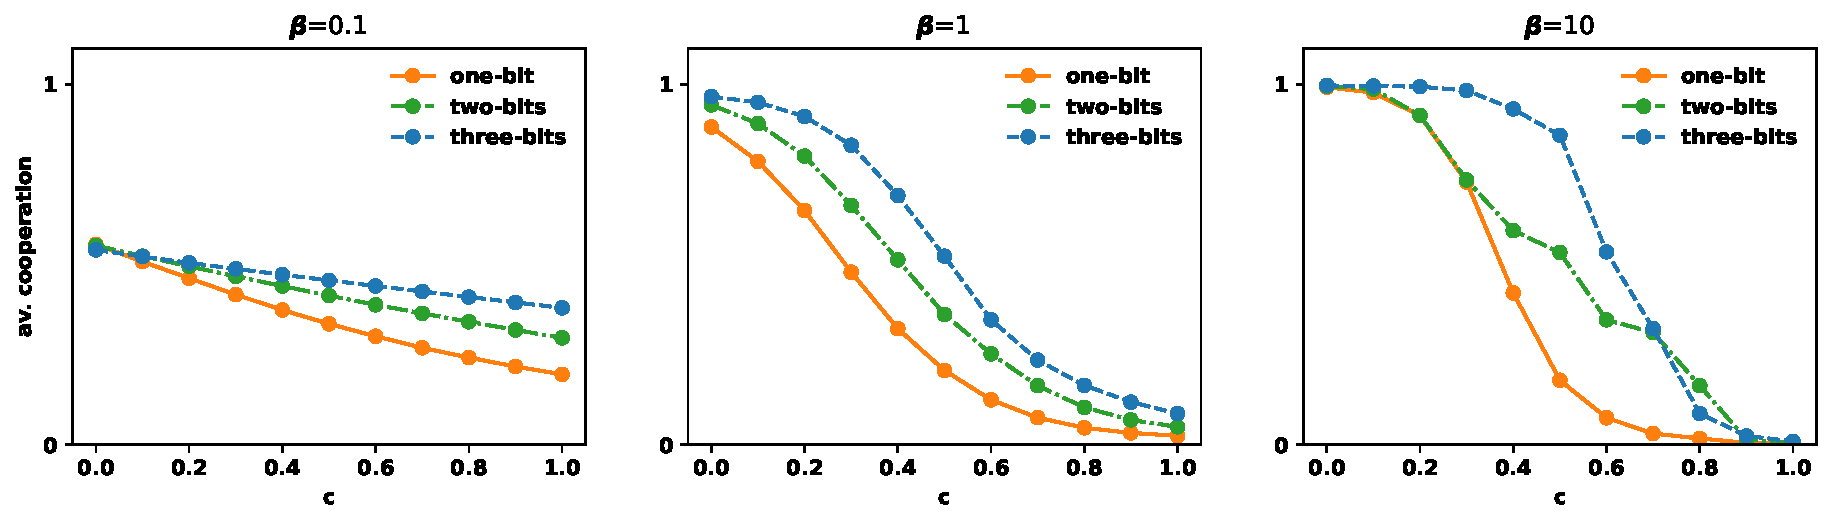
\includegraphics[width=\textwidth]{static/average_cooperation_over_c_with_diff_selection_strength.pdf}
  \end{subfigure}
  \hfill
  \begin{subfigure}{0.85\textwidth}
      \centering
      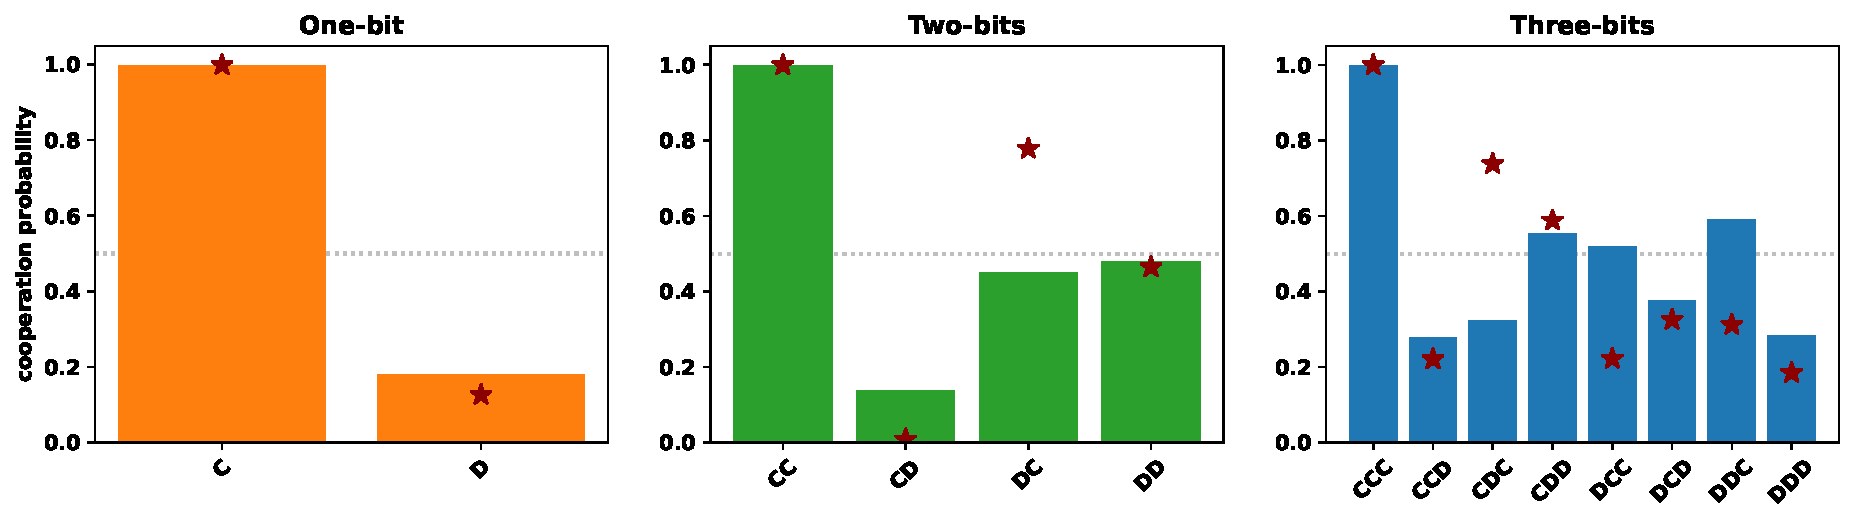
\includegraphics[width=\textwidth]{static/evolution_results_barplots.pdf}
  \end{subfigure}
  \hfill
  \begin{subfigure}{0.85\textwidth}
      \centering
      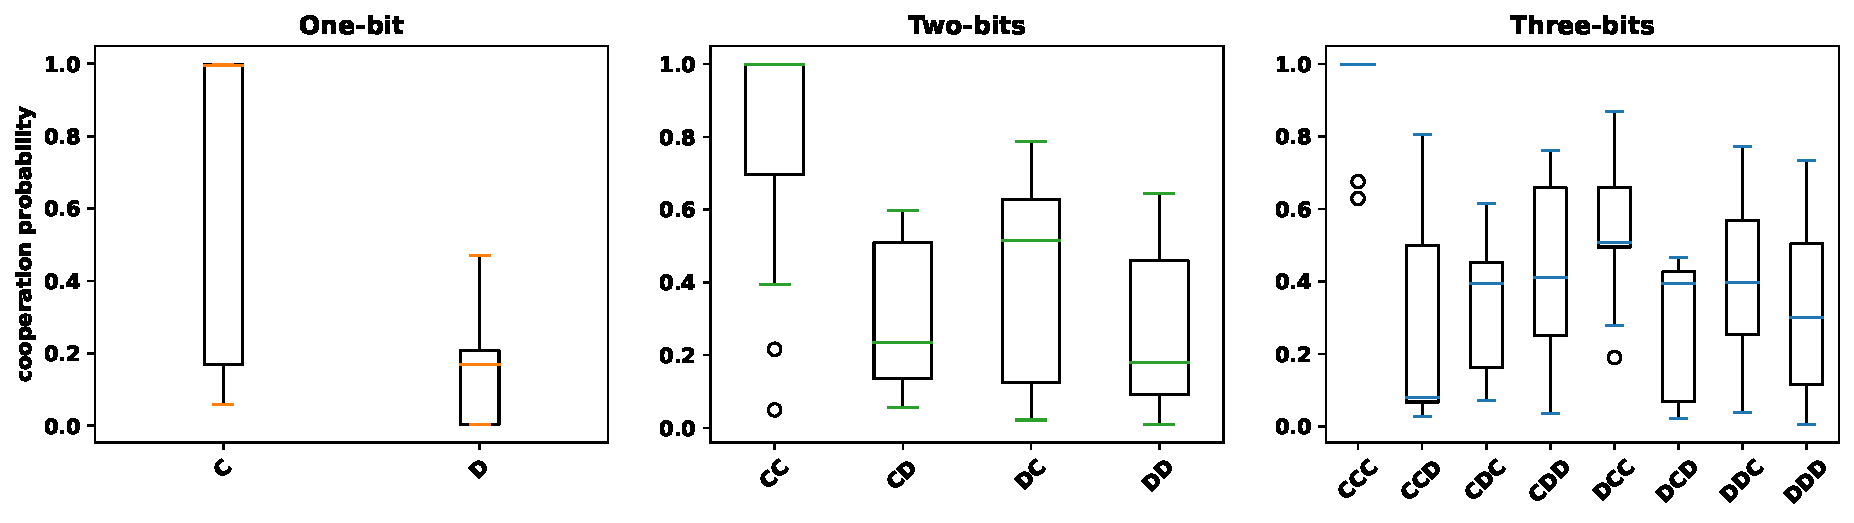
\includegraphics[width=\textwidth]{static/evolution_results_boxplots.pdf}
  \end{subfigure}
  \caption{\textbf{Comparing the evolving cooperation rates and the most
  abundant strategies  one-bit, two-bits, and three-bits strategies.}
  \textbf{A.} the evolving cooperation rates for different selection strengths.
  To assess the impact of memory on the evolution of cooperation, we ran
  simulations based on Imhof and Nowak for different benefit-to-cost ratios and
  different selection strengths. The average cooperation is calculated by
  considering the cooperation rate within the resident population. For a single
  run of the evolutionary process, we record the cooperating probabilities of
  the resident at each elementary time step. For each resident we estimate the
  cooperation rate between two resident strategies, and we take the average of
  that. 
  \textbf{B and C.} We ran 10 independent simulations for each set of strategies
  and recorded the most abundant strategy for each run. The abundant strategy is
  the resident that was fixed for the most time steps. For the simulations we
  used \(b=3 \text{ and } c=1\). The colored bars show the average values of
  cooperation probabilities of the most abundant strategies. The stars show the
  cooperation probabilities of the most abundant strategy for each set. The
  boxplots illustrate the distributions of cooperation probabilities for the ten
  runs.
  Parameters: \(N=100\), \(\beta=1\). Each simulation was run for \(10 ^ {5}\)
  mutant strategies except for the simulations where \(\beta=10\). These we
  run for \(2 \cdot 10 ^ {5}\).}\label{fig:three_graphs}
\end{figure}

\nikoleta{We ran these without error. Do we want to incooperate error in the
evolutionary simulations?}

\section{Conclusion}

In this work we have studied the space of \(n-\)bit reactive strategies. This
space was originally explored by the work of~\citep{nowak:AAM:1990}. The
reactive space contains many well known strategies from the literature, such as
Alternator, Grudger, Tif For Tat and Generous Tit For Tat. However, note that
these are reactive strategies of memory size one. We referred to these as
one-bit reactive strategies. Here we aimed to explore higher memory reactive
strategies, and even though this has been done previously for memory-\(n\)
strategies, many questions still remain open in the case of reactive ones.

In section~\ref{section:good_nash_strategies} we analytically explored two-bit
reactive strategies. We built on the work of~\citep{akin:EGADS:2016} and proved
that there is a set of stochastic two-bit strategies that can sustain
cooperative Nash equilibria. We verified our results with numerical simulations,
and showed that in the space of two-bit strategies (for the donation game) one
is Nash if it's Nash against AllD and (0, 1, 1, 0).

However, in the case of pure reactive strategies we showed that when there is a
vanishingly small probability of error, no cooperative Nash is possible. We
built on the work of~\citep{hilbe:PNAS:2017} where they numerically showed that
memory-\(n\) cooperative Nash are feasible. Thus, we can see that constraining
the information a strategy receives to only the co-players moves makes it harder
for cooperation.

In the last section~\ref{section:evolutionary_simulations}, we explored the
space of reactive strategies with evolutionary simulations. Though cooperative
Nash can be obtained, here we asked the question: can they also evolve? In all
the cases we have presented, high levels of cooperation can be achieved.

\appendix

% \section{Two-bit reactive strategies cheat sheet.}

% \begin{table}[!htbp]
%   \centering
%    \begin{tabular}{c c c c c c c }
%   \toprule
%    History/State & State number & Coop/Def & Coop. probability M. & Coop. probability & Reaction to & \\
%    \toprule
%   $CC|CC$  & 1 & Coop  & $p_1$ & $p_1$ & $CC$\\
%   $CC|CD$  & 2 & Coop  & $p_2$ & $p_2$ & $CD$ \\
%   $CC|DC$  & 3 & Def   & $p_3$ & $p_1$ & $CC$ \\
%   $CC|DD$  & 4 & Def   & $p_4$ & $p_2$ & $CD$ \\
%   $CD|CC$  & 5 & Coop  & $p_5$ & $p_3$ & $DC$ \\
%   $CD|CD$  & 6 & Coop  & $p_6$ & $p_4$ & $DD$ \\
%   $CD|DC$  & 7 & Def   & $p_7$ & $p_3$ & $DC$ \\
%   $CD|DD$  & 8 & Def   & $p_8$ & $p_4$ & $DD$ \\
%   $DC|CC$  & 9 & Coop  & $p_9$ & $p_1$ & $CC$ \\
%   $DC|CD$  & 10 & Coop & $p_{10}$ & $p_2$ & $CD$ \\
%   $DC|DC$  & 11 & Def  & $p_{11}$ & $p_1$ & $CC$ \\
%   $DC|DD$  & 12 & Def  & $p_{12}$ & $p_2$ & $CD$ \\
%   $DD|CC$  & 13 & Coop & $p_{13}$ & $p_3$ & $DC$ \\
%   $DD|CD$  & 14 & Coop & $p_{14}$ & $p_4$ & $DD$ \\
%   $DD|DC$  & 15 & Def  & $p_{15}$ & $p_3$ & $DC$ \\
%   $DD|DD$  & 16 & Def  & $p_{16}$ & $p_4$ & $DD$ \\
%   \hline
% \end{tabular}
% \caption{\textbf{Cheat Sheet} for two-bit reactive strategies.}
% \end{table}

\newpage

\bibliography{bibliography.bib}

\end{document}